\section{Intuition underlying the automatic implementation}
\label{sec:properties}

In this section, give the intuition on how we ensured that the implementation of
the hierarchical MSI protocol is correct.

The most important invariant that the generated protocol maintains between the
caches and its parent is as follows:
\begin{theorem}
Conservative: For two nodes $p, c$, where $p = c.parent$, $\forall a,
p.dir[c][a] \ge c.state[a]$.  \label{conservative}
\end{theorem}

This ensures that if a cache makes a decision about compatibility of states of
its children using the local directory information, then it does not violate the
compatibility of the children's real states. This essentially ensures that
reading the directory is sufficient to know the value of a cache's state.

Regarding the \send{} and \receive{} operations, the following
invariants are very critical to ensure that a thread completes. If they are not
true, then a thread might block waiting for a response, or being unable to send a
message, leading to a deadlock. Our generated protocol maintains this.

\begin{theorem}
It a thread has to send a message, it will eventually be able to send the
message.
\label{canSend}
\end{theorem}

\begin{theorem}
If a cache sends an upgrade-to-$x$ request to its parent, it will eventually
get an upgrade-to-$y$ response from the parent where $y \ge x$.
\label{willRecv}
\end{theorem}

\begin{theorem}
If a cache sends an downgrade-to-$x$ request to one of its children, it will
eventually get a downgrade-to-$y$ response from the child where $y \le x$.
\label{willRecv2}
\end{theorem}

Another scenario where a thread can potentially get suspended is if handling of
a request requires eviction of another cache line. The thread would get
suspended if all the lines that can be allocated for this request are being 
accessed by other suspended threads. But the generated protocol still guarantees
the following invariant.

\begin{theorem}
If a thread is waiting for a line to be allocated, \ie for any address to become
available for eviction, then some address will eventually become available for
eviction
\label{evictDead}
\end{theorem}

It this is not true, a thread that is waiting for being allocated a free line
may never proceed, leading to a deadlock.

If a cache receives a response message, it must know whether or not a) it will
be receiving data, and b) whether it has to update the address with the received
data, in case it does receive data. The first part can be indicated by the
message itself, but the second part has to be decided only after knowing the
state of the cache which sent the response. In this regard, the following two
invariants are very useful.

\begin{theorem}
If $p$ sends \Resp{p}{c}{a}{x} to $c$, where $p = c.parent$, then $p.dir[c][a]$
just before $p$ sends the response is the same as $c.state[a]$ just before $c$
receives the response.
\label{pcSame}
\end{theorem}

\begin{theorem}
If $c$ sends \Resp{c}{p}{a}{x} to $p$, where $p = c.parent$, then $c.state[a]$
just before $c$ sends the response is the same as $p.dir[c][a]$ just before $p$
receives the response.
\label{cpSame}
\end{theorem}

We will illustrate the need for Invariants \ref{pcSame}, \ref{cpSame} and
\ref{conservative} using an example of a 2-level system containing two L1
caches $c_1$ and $c_2$ with a shared L2 cache $p$.

Invariant \ref{pcSame} and \ref{cpSame} are important to make sure that the
data transfers happen correctly. Let $p.dir[c_1][a] = S$, $p.dir[c_2][a] = I$,
$c_1.state[a] = S$, and $c_2.state[a] = I$. $c_2$ gets a store request, and
sends an upgrade-to-$M$ request to $p$. $p$ receives the request, but assumes that
$c_1$ already has data for $a$ since $p.dir[c_1][a] = S$. Invariant
\ref{pcSame} is violated. So, it does not transfer the data to $c_1$, resulting
in $c_1$ waiting for data, and hence deadlock. A dual condition can be
constructed similarly, in which $c_1$ downgrades its state for address $a$ from
$S$ to $I$, and the parent assumes that $c_1$ is in state $M$, and keeps
waiting for data.

Invariant \ref{conservative} is important because a parent node consults its
directory to decide the children it needs to send a downgrade request to.  Let
$p.dir[c_1][a] = S$, $c_1.state[a] = S$, $p.dir[c_2][a] = I$ but
$c_2.state[a] = S$. If $c_1$ gets a store request from the processor and sends
an upgrade-to-$M$ request to $p$, $p$ will assume that $c_2$'s state for address $a$
is also $I$ and hence send an upgrade-to-$M$ response to $c_1$. But since the real
state of  $c_2$ for address $a$ is $S$, it will break Single-writer Invariant
\ref{singleWriter}.

Thus, if all the invariants above (\ref{conservative}, to \ref{cpSame}) hold,
then the threads given in Figure \ref{realistic} cannot deadlock because it
will always be able to a) send a request, b) send back a response, c) get back
a response for a request it sent, d) receive data when required. Though the
threads executing in a cache are actually suspensive, these invariants give an

We will show some of the core properties that are extracted
from the requirements spelt out in Section \ref{sec:DistributedMsi} and the
specification of the protocol (Figures \ref{msi-template} and
\ref{realistic}). These properties alone can be used to prove the above
invariants (Invariants \ref{conservative} to \ref{cpSame}). We do not present
the proof here, but give some intuition. Figure \ref{sendReq} lists these local
properties.

\floatstyle{boxed}
\restylefloat{figure}

\begin{figure}\small
\begin{inv}
A response \Resp{p}{c}{a}{x}, where $p = c.parent$, can be sent from $p$ only
if
\begin{enumerate}
\item a request \Req{c}{p}{a}{z} was received from $c$,
\item $p$ is not waiting for any response for address $a$ from $c$, and
\item $x > y$, where $p.dir[c][a] = y$ just before sending the response
\end{enumerate}
\label{pSendRespPre}
\end{inv}
\begin{inv}
A response \Resp{c}{p}{a}{x}, where $p = c.parent$, can be sent from $c$ only
if $x < y$, where $c.state[a] = y$ just before sending the
response\label{cSendRespPre1}
\end{inv}
\begin{inv}
If $c$ has sent a request \Req{c}{p}{a}{x}, then $c$ can send a response
\Resp{c}{p}{a}{y} only on receiving a request from $p$ for address $a$.
\label{cSendRespPre2}
\end{inv}
\caption{Local-Properties for sending responses}
\label{sendResp}
\end{figure}

The properties in Figure \ref{sendResp} restrict when responses can be sent by
 a cache (either to its children or to its parent).

\begin{figure}\small
\begin{inv}
If a response \Resp{p}{c}{a}{x} is sent from $p$, then $p.dir[c][a] \gets x$\label{cSendRespPost}
\end{inv}
\begin{inv}
If \Resp{c}{p}{a}{x} is sent $c.state[a] \gets x$\label{pSendRespPost}
\end{inv}
\begin{inv}
On receiving a response \Resp{c}{p}{a}{x}, where $p = c.parent$, $p.dir[c][a]
\gets x$\label{pRecvResp}
\end{inv}
\begin{inv}
On receiving a response \Resp{p}{c}{a}{x}, where $p = c.parent$, $c.state[c]
\gets x$\label{cRecvResp}
\end{inv}
\begin{inv}
$c.state[a]$ can change only on $c$ sending a response to or receiving a
response from $c.parent$\label{cState}
\end{inv}
\begin{inv}
$p.dir[c][a]$ can change only on $p$ sending or receiving a response from
its child $c$\label{pState}
\end{inv}
\caption{Local-Properties for state changes}
\label{stateChange}
\end{figure}

The properties in Figure \ref{stateChange} specify exactly when the coherence state of
a line (both directory and state) changes.

\begin{figure}\small
\begin{inv}
\Req{p}{c}{a}{x}, where $p = c.parent$, can be sent only if $x < p.dir[c][a]$\label{pSendReqPre}
\end{inv}
\begin{inv}
If \Req{p}{c}{a}{x}, where $p = c.parent$, is received, if $x \ge c.state[a]$,
then the request is dropped\label{pSendReqPost}
\end{inv}
\begin{inv}
\Req{c}{p}{a}{x}, where $p = c.parent$, can be sent only if $x > c.state[a]$\label{cSendReqPre}
\end{inv}
\begin{inv}
If \Req{c}{p}{a}{x}, where $p = c.parent$, is received, it $x \le p.state[a]$,
then the request is dropped\label{cSendReqPost}
\end{inv}
\begin{inv}
A request can be sent by a cache node $n$ for address $n$ to another cache node $m$ only if
node $n$ is not waiting for a response for address $a$ from $m$.
\label{nodoublereq}
\end{inv}
\caption{Local-Properties useful in proving the correctness of MSI protocol}
\label{sendReq}
\end{figure}

 We will use the violation of Local-Properties \ref{pSendRespPre} and
\ref{cSendRespPre2} as examples to illustrate the importance of local
properties.  In our usual system, let's say $c_1.state[a] = p.dir[c_1][a] = S$,
$c_2.state[a] = p.dir[c_2][a] = I$.

\floatstyle{plain}
\restylefloat{figure}
\begin{figure}
\centering
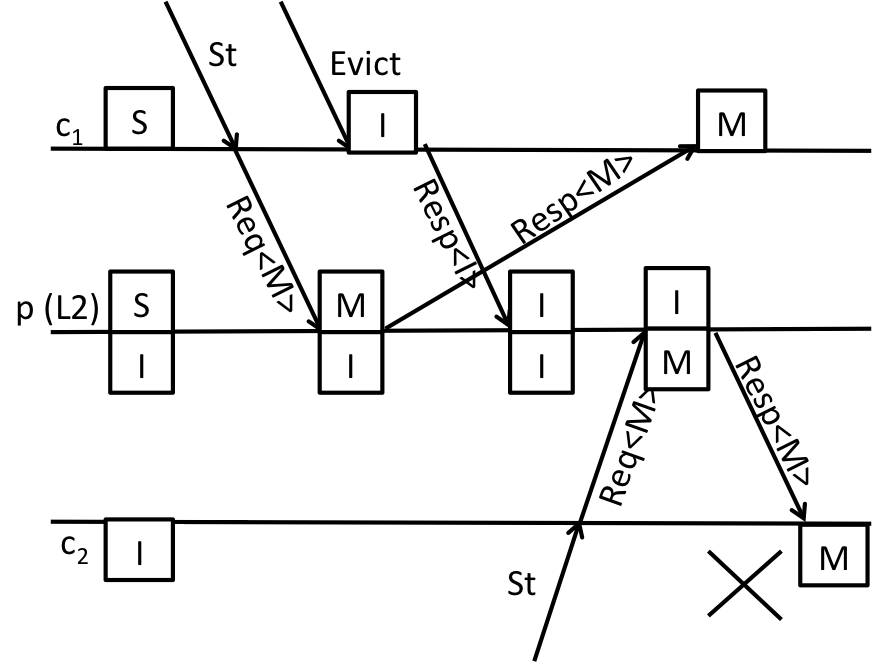
\includegraphics[scale=0.4]{checkit}
\caption{Effect of violating Local-Property \ref{cSendRespPre2} (child evicts a ``pending'' line)}
\label{checkit}
\end{figure}
\floatstyle{boxed}
\restylefloat{figure}

Let $c_1$ receive a store request for address $a$. It sends an upgrade-to-$M$
request to $p$. Then $c_1$ violates \ref{cSendRespPre2} and evicts $a$ to
replace it with another address. It sends a downgrade to $I$ response for
address $a$ to $p$.  Meanwhile $p$ has sent an upgrade-to-$M$ response to
$c_1$. $c_1$ receives the response and upgrades address $a$ to $M$. $p$ then
receives the downgrade to $I$ response form $c_1$. So $p$ now assumes that
$c_1$ is in $I$ while in reality, $c_1$ is in $M$. This breaks Invariant
\ref{conservative} which creates the problems described earlier. This is shown
in Figure \ref{checkit}

\floatstyle{plain}
\restylefloat{figure}
\begin{figure}
\centering
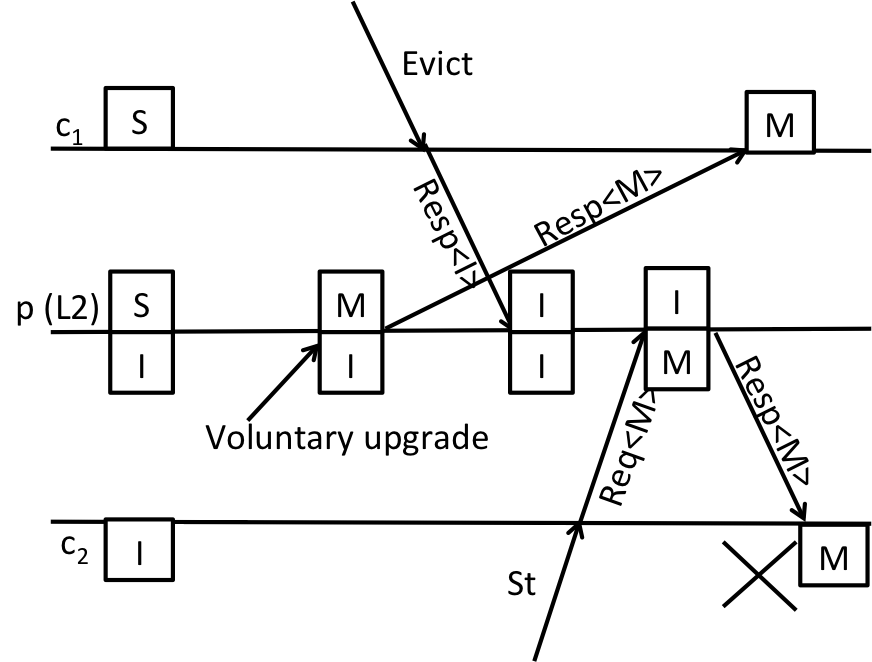
\includegraphics[scale=0.4]{checkit2}
\caption{Effect of violating Local-Property \ref{pSendRespPre} (parent sends a voluntary response)}
\label{checkit2}
\end{figure}
\floatstyle{boxed}
\restylefloat{figure}

Let's say $p$ violates \ref{pSendRespPre} and voluntarily sends an
upgrade-to-$M$ response for address $a$ to $c_1$.  Meanwhile, $c_1$ evicts $a$
to replace it with another address. $c_1$ then gets the upgrade-to-$M$ response
from $p$ while $p$ gets the downgrade to $I$ response, breaking Invariant
\ref{conservative} again. This is shown in Figure \ref{checkit2}.

In general, any if response messages from both a cache to its parent and from
the parent to the same cache are in flight together, like the scenarios in
Figures \ref{checkit} and \ref{checkit2} Invariant \ref{conservative} will be
violated.

\begin{figure}
\begin{subfigure}{.25\linewidth}
\centering
\begin{tabular}{|ccc|}
\hline
$M$ & $\rightarrow$ & $I$\\
$O$ & $\rightarrow$ & $S$\\
$S$ & $\rightarrow$ & $O$\\
$I$ & $\rightarrow$ & $I$\\
\hline
\end{tabular}
\subcaption*{$toCompatible$}
\end{subfigure}
\begin{subfigure}{.25\linewidth}
\centering
\begin{tabular}{|c|c|}
\hline
$M$ & $\checkmark$\\
$O$ & $\checkmark$\\
$S$ & $\times$\\
$I$ & $\times$\\
\hline
\end{tabular}
\subcaption*{$dataToUpper$}
\end{subfigure}
\begin{subfigure}{.48\linewidth}
\centering
\begin{tabular}{|c|cccc|}
\hline
& $M$ & $O$ & $S$ & $I$\\
\hline
$M$ & $=$ & $>$ & $>$ & $>$\\
$O$ & $<$ & $=$ & $>$ & $>$\\
$S$ & $<$ & $<$ & $=$ & $>$\\
$I$ & $<$ & $<$ & $<$ & $=$\\
\hline
\end{tabular}
\subcaption*{$<$ (and other) relations}
\end{subfigure}
\caption{MOSI protocol mappings and $<$ relations}
\label{mosi}
\end{figure}

These properties do not require messages to physically come from the sources as
indicated by the requests or responses -- some other cache node can forward
these messages. These can be used to generalize our procedure to
cache-intervention based protocols like MOSI. We generalize the states of MOSI
using the $<$ relation and auxiliary functions $maxCompatible$ and $isModified$,
as shown in Figure \ref{mosi}. 

In a hierarchical setting for the MOSI protocol, any cache can send data
with the response granting permissions to the requesting L1 cache, instead of
going through the hierarchy.  On a load request, L1 cache $c$ sends an
upgrade-to-$O$ request, instead of an upgrade-to-$S$ request. The request keeps
going up the hierarchy, sending an upgrade-to-$O$ request to each of the parent
on the way, till it reaches a cache $p$ which has that line in $M$ or $O$
state. If some other child is in $O$ or $M$ state, this node sends a
upgrade-$c$-to-$O$ in addition to a downgrade-to-$S$ request to that cache.
This upgrade-$c$-to-$O$ + downgrade-to-$S$ keeps propagating down the tree till
it reaches a node $n$ whose children are all in a state $< O$. $n$ then
downgrades its state, forwards the upgrade-to-$O$ response to $c$ and
simultaneously sends a fwd-and-downgrade-to-$S$ response to its parent, which
keeps forwarding that till it reaches $p$. If $c$ gets a store request, it will
send an upgrade-to-$M$ request, and $p$ would send a downgrade-to-$I$ request
instead, to its children.

The caches encountered on the way from $n$ to $p$ should handle an extra
scenario where it gets a downgrade response, without a forward response.In this
case, the data and permission forwarding has to be done from this cache to $c$.
It is the designer's responsibility to ensure that this case is handled. 

This protocol obeys all the local properties and the requirements mentioned in
this section except that a request sent to a cache might overtake a response
forwarded to that cache. To avoid this, once the forwarding message is
delivered to the intended destination ($c$ in our case), then $c$ sends back an
ACK. $c$'s parent is allowed to start sending downgrade requests for that
address only after receiving this ACK. This ACK is sent back to each of the
parents till it reaches $p$, which allows each of these caches to send
downgrade requests for that address towards $c$.  This satisfies all the
requirements of Section \ref{sec:DistributedMsi} and the local properties given in
Figures \ref{sendResp}, \ref{stateChange} and \ref{sendReq}, thereby automatically being correct. The reasoning for
its correctness gets localized to checking if the ordering Requirement
\ref{reqNoOvertakeResp} is maintained.

The protocols can also be extended in a different dimension. The proof is
oblivious to the states, so any downgrade of a state is treated the same. This
means that a cache line can downgrade from $M$ to $S$ state instead of going all
the way down to $I$ state. This flexibility can potentially be exploited, and we
will study its effects in the future.
